\input{header.tex}
\input{newcommands.tex}

% Optionsfelder (radio) brauchen unicode=false, sonst bekommen sie kaputte Namen
\hypersetup{unicode=false, pdftitle={Ausfüllbare PDF-Formulare mit LaTeX}}

\title{Ausfüllbare PDF-Formulare mit \hologo{LaTeX} erstellen}
\author{Fortbildungsmaterial für MINT-Lehrkräfte}
\date{\today}
\pagestyle{plain}
\setlength{\parskip}{1.5em}

\begin{document}
\begin{Form}

\maketitle

Ein Arbeitsblatt oder eine Leistungskontrolle, die Schülerinnen und Schüler
direkt am Tablet oder Laptop ausfüllen, speichern und über die Lernplattform
zurückgeben: Dafür braucht man kein Zusatzprogramm. \hologo{LaTeX} kann mit dem
Paket \texttt{hyperref} echte PDF-Formularfelder erzeugen, also Textfelder,
Ankreuzkästchen, Optionsfelder und Auswahllisten. Diese Handreichung zeigt
Schritt für Schritt, wie das geht, und baut am Ende eine vorhandene
Papier-Leistungskontrolle zu einer digitalen Fassung um. Ausgewertet wird
dabei nichts automatisch: Die Lehrkraft liest jede Abgabe selbst, wie bei
Papier auch. Die Felder in den blauen Ausgabe-Kästen dieser Handreichung sind
echt. Sie können sie im PDF direkt ausprobieren.



%%%%  KAPITEL 1  %%%%
\section{Grundlagen und benötigte Pakete}

%%%%  UNTERKAPITEL 1.1  %%%%
\subsection{Was man braucht}

Formularfelder gehören zum Paket \texttt{hyperref}. Es ist in der universalen
\texttt{header.tex} bereits geladen. Zwei Dinge kommen für ein Formular dazu:

\begin{itemize}
	\item Alle Felder stehen innerhalb der Umgebung \texttt{Form}. Am
	einfachsten umschließt sie den ganzen Inhalt, direkt nach
	\verb|\begin{document}| bis direkt vor \verb|\end{document}|.
	\item In der Präambel steht \verb|\hypersetup{unicode=false}|. Das ist nur
	für Optionsfelder (Kapitel~3.3) nötig, schadet aber den anderen Feldern
	nicht. Ohne diese Zeile erzeugt \texttt{hyperref} (getestet mit Version
	7.01h) für Optionsfelder unlesbare interne Namen.
\end{itemize}

Das Grundgerüst eines Formulars sieht damit so aus:

\begin{lstlisting}[style=latex]
\input{header.tex}
\input{newcommands.tex}
\hypersetup{unicode=false}

\begin{document}
\begin{Form}

  ... Aufgaben mit Feldern ...

\end{Form}
\end{document}
\end{lstlisting}


Kompiliert wird wie immer mit \texttt{pdflatex}. JavaScript oder besondere
Programme sind nicht nötig.

%%%%  UNTERKAPITEL 1.2  %%%%
\subsection{Die Feldtypen im Überblick}

\renewcommand{\arraystretch}{1.3}
\begin{tabular}{p{4.6cm} p{11cm}}
	\toprule
	\textbf{Befehl} & \textbf{Wofür} \\
	\midrule
	\verb|\TextField| & Textfeld, ein- oder mehrzeilig \\
	\verb|\CheckBox| & Ankreuzkästchen, unabhängig von anderen \\
	\verb|\ChoiceMenu[radio]| & Optionsfelder: genau eine Antwort aus mehreren \\
	\verb|\ChoiceMenu|\newline\verb|  [combo, popdown]| & Auswahlliste zum Aufklappen \\
	\verb|\Reset| & Knopf, der alle Felder leert (für Leistungskontrollen ungeeignet, siehe Kapitel 8) \\
	\bottomrule
\end{tabular}

Für den Schulalltag stehen in der universalen \texttt{newcommands.tex} vier
Kurzbefehle bereit, die auf diesen Feldern aufbauen: \verb|\feld|,
\verb|\zeichen|, \verb|\kreuz| und \verb|\antwort|. Sie werden in den
folgenden Kapiteln vorgestellt.



%%%%  KAPITEL 2  %%%%
\section{Textfelder}

%%%%  UNTERKAPITEL 2.1  %%%%
\subsection{Ein erstes Textfeld}

Jedes Feld braucht einen \textbf{Namen}. Unter diesem Namen speichert das PDF
später die Eingabe. Die leeren geschweiften Klammern am Ende sind die
Beschriftung, die \texttt{hyperref} vor das Feld setzen würde. Wir lassen sie
leer und schreiben die Beschriftung selbst davor:

\begin{lstlisting}[style=latex]
Name: \TextField[name=bsp-name, width=6cm]{}
\end{lstlisting}

\begin{ausgabe}
Name: \TextField[name=bsp-name, width=6cm]{}
\end{ausgabe}


Die Breite legt \texttt{width} fest. Ohne Angabe ist das Feld 3\,cm breit. Der
blaue Rand und der hellblaue Hintergrund kommen aus der
\texttt{newcommands.tex} (Kapitel 4), ebenso die Schriftgröße 11\,pt für das,
was eingetippt wird.

%%%%  UNTERKAPITEL 2.2  %%%%
\subsection{Größe, Schrift und Vorbelegung}

Mit \texttt{height} wird das Feld höher, mit \texttt{charsize} die Schrift
größer. \texttt{value} trägt einen Text vor, den man überschreiben kann, zum
Beispiel die Klasse:

\begin{lstlisting}[style=latex]
Klasse: \TextField[name=bsp-klasse, width=2cm, value={10b}]{} \qquad
Ort: \TextField[name=bsp-ort, width=5cm, height=0.9cm, charsize=16pt]{}
\end{lstlisting}

\begin{ausgabe}
Klasse: \TextField[name=bsp-klasse, width=2cm, value={10b}]{} \qquad
Ort: \TextField[name=bsp-ort, width=5cm, height=0.9cm, charsize=16pt]{}
\end{ausgabe}


Hier sieht man auch einen Schönheitsfehler: Ein Feld sitzt mit seiner
Unterkante auf der Grundlinie und ragt deshalb über den Text hinaus. Im
nächsten Abschnitt wird das gelöst.

%%%%  UNTERKAPITEL 2.3  %%%%
\subsection{Lücken im Satz: \texttt{\textbackslash feld}}

Der Kurzbefehl \verb|\feld[Breite]{Name}| setzt ein Textfeld etwas tiefer,
sodass der eingetippte Text auf derselben Linie steht wie der Satz. Er
ersetzt die Schreiblücke eines Papierblatts:

\begin{lstlisting}[style=latex]
Der Operator \texttt{//} heißt \feld[4cm]{bsp-op1}, der Operator
\texttt{\%} heißt \feld[4cm]{bsp-op2}.
\end{lstlisting}

\begin{ausgabe}
Der Operator \texttt{//} heißt \feld[4cm]{bsp-op1}, der Operator
\texttt{\%} heißt \feld[4cm]{bsp-op2}.
\end{ausgabe}


Ohne Breitenangabe ist das Feld 2,4\,cm breit. Wichtig ist der Name: Er muss
im ganzen Dokument eindeutig sein. Mehr dazu in Kapitel 4.3.

%%%%  UNTERKAPITEL 2.4  %%%%
\subsection{Genau ein Zeichen: \texttt{\textbackslash zeichen}}

Für Zuordnungen mit einem Buchstaben (E, V oder A; die Reihenfolge von
Programmzeilen) gibt es \verb|\zeichen{Name}|. Das Feld nimmt nur ein Zeichen
an (\texttt{maxlen=1}) und zeigt es zentriert (\texttt{align=1}):

\begin{lstlisting}[style=latex]
Reihenfolge: \zeichen{bsp-r1}\ \zeichen{bsp-r2}\ \zeichen{bsp-r3}\
\zeichen{bsp-r4}
\end{lstlisting}

\begin{ausgabe}
Reihenfolge: \zeichen{bsp-r1}\ \zeichen{bsp-r2}\ \zeichen{bsp-r3}\
\zeichen{bsp-r4}
\end{ausgabe}


%%%%  UNTERKAPITEL 2.5  %%%%
\subsection{Mehrzeilige Antworten: \texttt{\textbackslash antwort}}

Wo auf Papier Schreiblinien stehen, braucht man ein mehrzeiliges Feld. Der
Grundbefehl ist ein \verb|\TextField| mit \texttt{multiline=true}:

\begin{lstlisting}[style=latex]
\TextField[name=bsp-frei, multiline=true, width=12cm, height=2cm]{}
\end{lstlisting}

\begin{ausgabe}
\TextField[name=bsp-frei, multiline=true, width=12cm, height=2cm]{}
\end{ausgabe}


Bequemer ist \verb|\antwort[Höhe]{Name}|. Das Feld beginnt in einer neuen
Zeile, nimmt die ganze Zeilenbreite ein und ist ohne Angabe 3,2\,cm hoch. Das
entspricht etwa vier Schreiblinien und bietet bei 11\,pt Schrift Platz für
sechs bis sieben getippte Zeilen:

\begin{lstlisting}[style=latex]
Erkläre den Unterschied zwischen einem Syntaxfehler und einem
Semantikfehler.
\antwort[2.5cm]{bsp-fehler}
\end{lstlisting}

\begin{ausgabe}
Erkläre den Unterschied zwischen einem Syntaxfehler und einem
Semantikfehler.
\antwort[2.5cm]{bsp-fehler}
\end{ausgabe}


Zeilenumbrüche mit der Eingabetaste sind in mehrzeiligen Feldern erlaubt. Wird
mehr getippt, als hineinpasst, scrollt das Feld. Beim Ausdrucken fehlt der
überstehende Text dann allerdings, deshalb die Felder lieber großzügig planen.



%%%%  KAPITEL 3  %%%%
\section{Ankreuzen und Auswählen}

%%%%  UNTERKAPITEL 3.1  %%%%
\subsection{Ankreuzkästchen: \texttt{\textbackslash kreuz}}

\verb|\CheckBox| erzeugt ein Kästchen, das per Klick ein Häkchen bekommt.
\verb|\kreuz{Name}| ist dasselbe in passender Größe und Höhe für den
Fließtext:

\begin{lstlisting}[style=latex]
Kreuze an, welche Zeile zur Verarbeitung gehört.\\
\kreuz{bsp-z1}\ Zeile 1 \qquad \kreuz{bsp-z2}\ Zeile 2 \qquad
\kreuz{bsp-z3}\ Zeile 3
\end{lstlisting}

\begin{ausgabe}
Kreuze an, welche Zeile zur Verarbeitung gehört.\\
\kreuz{bsp-z1}\ Zeile 1 \qquad \kreuz{bsp-z2}\ Zeile 2 \qquad
\kreuz{bsp-z3}\ Zeile 3
\end{ausgabe}


Jedes Kästchen ist ein eigenes Feld. Man kann also auch mehrere ankreuzen, so
wie auf Papier. Für Aufgaben wie \enquote{Kreuze alle richtigen Aussagen an}
ist das genau richtig.

%%%%  UNTERKAPITEL 3.2  %%%%
\subsection{Kästchen in Tabellen}

Richtig-falsch-Tabellen und Zuordnungen funktionieren genauso, das Kästchen
steht einfach in der Tabellenzelle:

\begin{lstlisting}[style=latex]
\begin{tabular}{p{7.5cm}cc}
  \toprule
  Aussage & richtig & falsch \\
  \midrule
  \texttt{"7"} ist eine Zahl. & \kreuz{bsp-k1r} & \kreuz{bsp-k1f} \\
  \texttt{2.0} ist ein \texttt{float}. & \kreuz{bsp-k2r} & \kreuz{bsp-k2f} \\
  \bottomrule
\end{tabular}
\end{lstlisting}

\begin{ausgabe}
\begin{tabular}{p{7.5cm}cc}
  \toprule
  Aussage & richtig & falsch \\
  \midrule
  \texttt{"7"} ist eine Zahl. & \kreuz{bsp-k1r} & \kreuz{bsp-k1f} \\
  \texttt{2.0} ist ein \texttt{float}. & \kreuz{bsp-k2r} & \kreuz{bsp-k2f} \\
  \bottomrule
\end{tabular}
\end{ausgabe}


Dass das so ordentlich aussieht, liegt an einer Kleinigkeit in
\verb|\kreuz|: Das Kästchen steckt in einer eigenen Box
(\verb|\raisebox|). Ein nacktes \verb|\CheckBox| übernimmt in einer Tabelle die
Höhe der ganzen Zeile und wird zu einem langen, schmalen Rechteck. Dasselbe
gilt für Textfelder. Alle vier Kurzbefehle sind deshalb so gebaut.

%%%%  UNTERKAPITEL 3.3  %%%%
\subsection{Optionsfelder: genau eine Antwort}

Soll nur eine Antwort möglich sein, nimmt man Optionsfelder. Klickt man ein
anderes an, verschwindet die erste Markierung. Alle Optionen gehören zu
\emph{einem} \verb|\ChoiceMenu| mit dem Schlüssel \texttt{radio}. Die Liste am
Ende hat die Form \texttt{Beschriftung=Wert}:

\begin{lstlisting}[style=latex]
\texttt{2.0} hat den Datentyp
\ChoiceMenu[radio, name=bsp-typ, default=]{}{int=int,
  float=float, str=str}
\end{lstlisting}

\begin{ausgabe}
\texttt{2.0} hat den Datentyp
\ChoiceMenu[radio, name=bsp-typ, default=]{}{int=int,
  float=float, str=str}
\end{ausgabe}


Die Beschriftung steht dabei immer \emph{vor} dem Knopf. \texttt{default=}
(leer) sorgt dafür, dass anfangs nichts ausgewählt ist. Der Wert hinter dem
Gleichheitszeichen ist das, was später gespeichert wird.

Optionsfelder brauchen \verb|\hypersetup{unicode=false}| in der Präambel
(siehe Kapitel 1.1). Und sie stehen immer in einer Reihe nebeneinander. Für
Tabellen mit Spalten \enquote{richtig} und \enquote{falsch} nimmt man deshalb
besser Kästchen wie in Kapitel 3.2.

%%%%  UNTERKAPITEL 3.4  %%%%
\subsection{Auswahllisten}

Eine Auswahlliste klappt beim Anklicken auf. Sie spart Platz und verhindert
Tippfehler, zum Beispiel bei E, V oder A:

\begin{lstlisting}[style=latex]
Der Automat berechnet das Wechselgeld.
\ChoiceMenu[combo, popdown, name=bsp-eva, width=1.6cm]{}{E,V,A}
\end{lstlisting}

\begin{ausgabe}
Der Automat berechnet das Wechselgeld.
\ChoiceMenu[combo, popdown, name=bsp-eva, width=1.6cm]{}{E,V,A}
\end{ausgabe}


Es braucht beide Schlüssel: \texttt{popdown} allein erzeugt eine fest
aufgeklappte Liste, \texttt{combo} allein ein Feld, in das man auch frei
tippen kann. Anfangs ist das Feld leer, eine Antwort entsteht erst durch die Auswahl
(getestet in Chrome). Auf Tablets sind Auswahllisten etwas umständlicher zu
bedienen als ein Feld für ein Zeichen. Für Leistungskontrollen ist
\verb|\zeichen| deshalb die robustere Wahl.



%%%%  KAPITEL 4  %%%%
\section{Einheitliches Aussehen und Feldnamen}

%%%%  UNTERKAPITEL 4.1  %%%%
\subsection{Standardwerte für alle Felder}

\texttt{hyperref} liest das Aussehen jedes Feldtyps aus einem
\verb|\DefaultOptionsof...|-Befehl. In der \texttt{newcommands.tex} sind diese
einmal für alle Dokumente festgelegt:

\begin{lstlisting}[style=latex]
\renewcommand{\DefaultOptionsofText}{print, bordercolor={0 0.353 0.612},
  backgroundcolor={0.94 0.96 1}, charsize=11pt}
\renewcommand{\DefaultOptionsofCheckBox}{print, bordercolor={0 0.353 0.612},
  backgroundcolor={0.94 0.96 1}, charsize=11pt}
\renewcommand{\DefaultHeightofText}{0.6cm}
\end{lstlisting}


Farben stehen hier nicht als Farbname, sondern als drei Zahlen zwischen 0 und
1 für Rot, Grün und Blau. \texttt{print} sorgt dafür, dass die Felder samt
Inhalt mitgedruckt werden. Wer ein Feld einmal anders haben möchte, gibt die
Option direkt beim Feld an, sie gilt dann nur dort:

\begin{lstlisting}[style=latex]
\TextField[name=bsp-rot, width=4cm, bordercolor={0.8 0 0},
  backgroundcolor={1 0.94 0.94}]{}
\end{lstlisting}

\begin{ausgabe}
\TextField[name=bsp-rot, width=4cm, bordercolor={0.8 0 0},
  backgroundcolor={1 0.94 0.94}]{}
\end{ausgabe}


%%%%  UNTERKAPITEL 4.2  %%%%
\subsection{Die vier Kurzbefehle}

So sind die Kurzbefehle in der \texttt{newcommands.tex} definiert:

\begin{lstlisting}[style=latex]
\newcommand{\feld}[2][2.4cm]{\raisebox{-0.17cm}{\TextField[name=#2, width=#1]{}}}
\newcommand{\zeichen}[1]{\raisebox{-0.12cm}{\TextField[name=#1, width=0.8cm,
  height=0.5cm, maxlen=1, align=1]{}}}
\newcommand{\kreuz}[1]{\raisebox{-0.08cm}{\CheckBox[name=#1, width=0.42cm,
  height=0.42cm]{}}}
\newcommand{\antwort}[2][3.2cm]{\par\vspace{0.15cm}\noindent
  \hbox{\TextField[name=#2, multiline=true, width=\linewidth, height=#1]{}}}
\end{lstlisting}


%%%%  UNTERKAPITEL 4.3  %%%%
\subsection{Feldnamen sinnvoll vergeben}

Der Name eines Feldes taucht für die Schülerinnen und Schüler nirgends auf.
Für die Lehrkraft ist er aber wichtig, sobald man Antworten einsammelt
(Kapitel 7). Bewährt hat sich ein Schema nach Aufgabennummer:

\begin{tabular}{ll}
	\texttt{name}, \texttt{klasse}, \texttt{datum} & Kopf des Blattes \\
	\texttt{a2-s3} & Aufgabe 2, Schritt 3 \\
	\texttt{a4-1-r}, \texttt{a4-1-f} & Aufgabe 4, Aussage 1, Spalte richtig/falsch \\
	\texttt{a5} & Aufgabe 5, freie Antwort \\
	\texttt{z-1} & Zusatzaufgabe, Lücke 1 \\
\end{tabular}

Zwei Regeln dazu, beide getestet:

\begin{itemize}
	\item \textbf{Bindestrich statt Unterstrich.} Ein Unterstrich im Namen
	wird von \texttt{hyperref} stillschweigend entfernt: Aus \texttt{a4\_1\_r}
	wird \texttt{a41r}.
	\item \textbf{Jeder Name nur einmal.} Zwei Felder mit demselben Namen
	behandelt nicht jedes Programm gleich. In Chrome sind es zwei getrennte
	Felder, andere Programme können sie zusammenlegen.
\end{itemize}



%%%%  KAPITEL 5  %%%%
\section{Praxis: eine Leistungskontrolle digital umbauen}

Als Beispiel dient eine Leistungskontrolle für Klasse 10 (Python-Grundlagen,
8 Aufgaben, 20 Punkte), die es bereits als Papierfassung gab. Die digitale
Fassung sieht gleich aus. Nur dort, wo auf Papier geschrieben oder angekreuzt
wird, steht jetzt ein Feld.

\begin{center}
	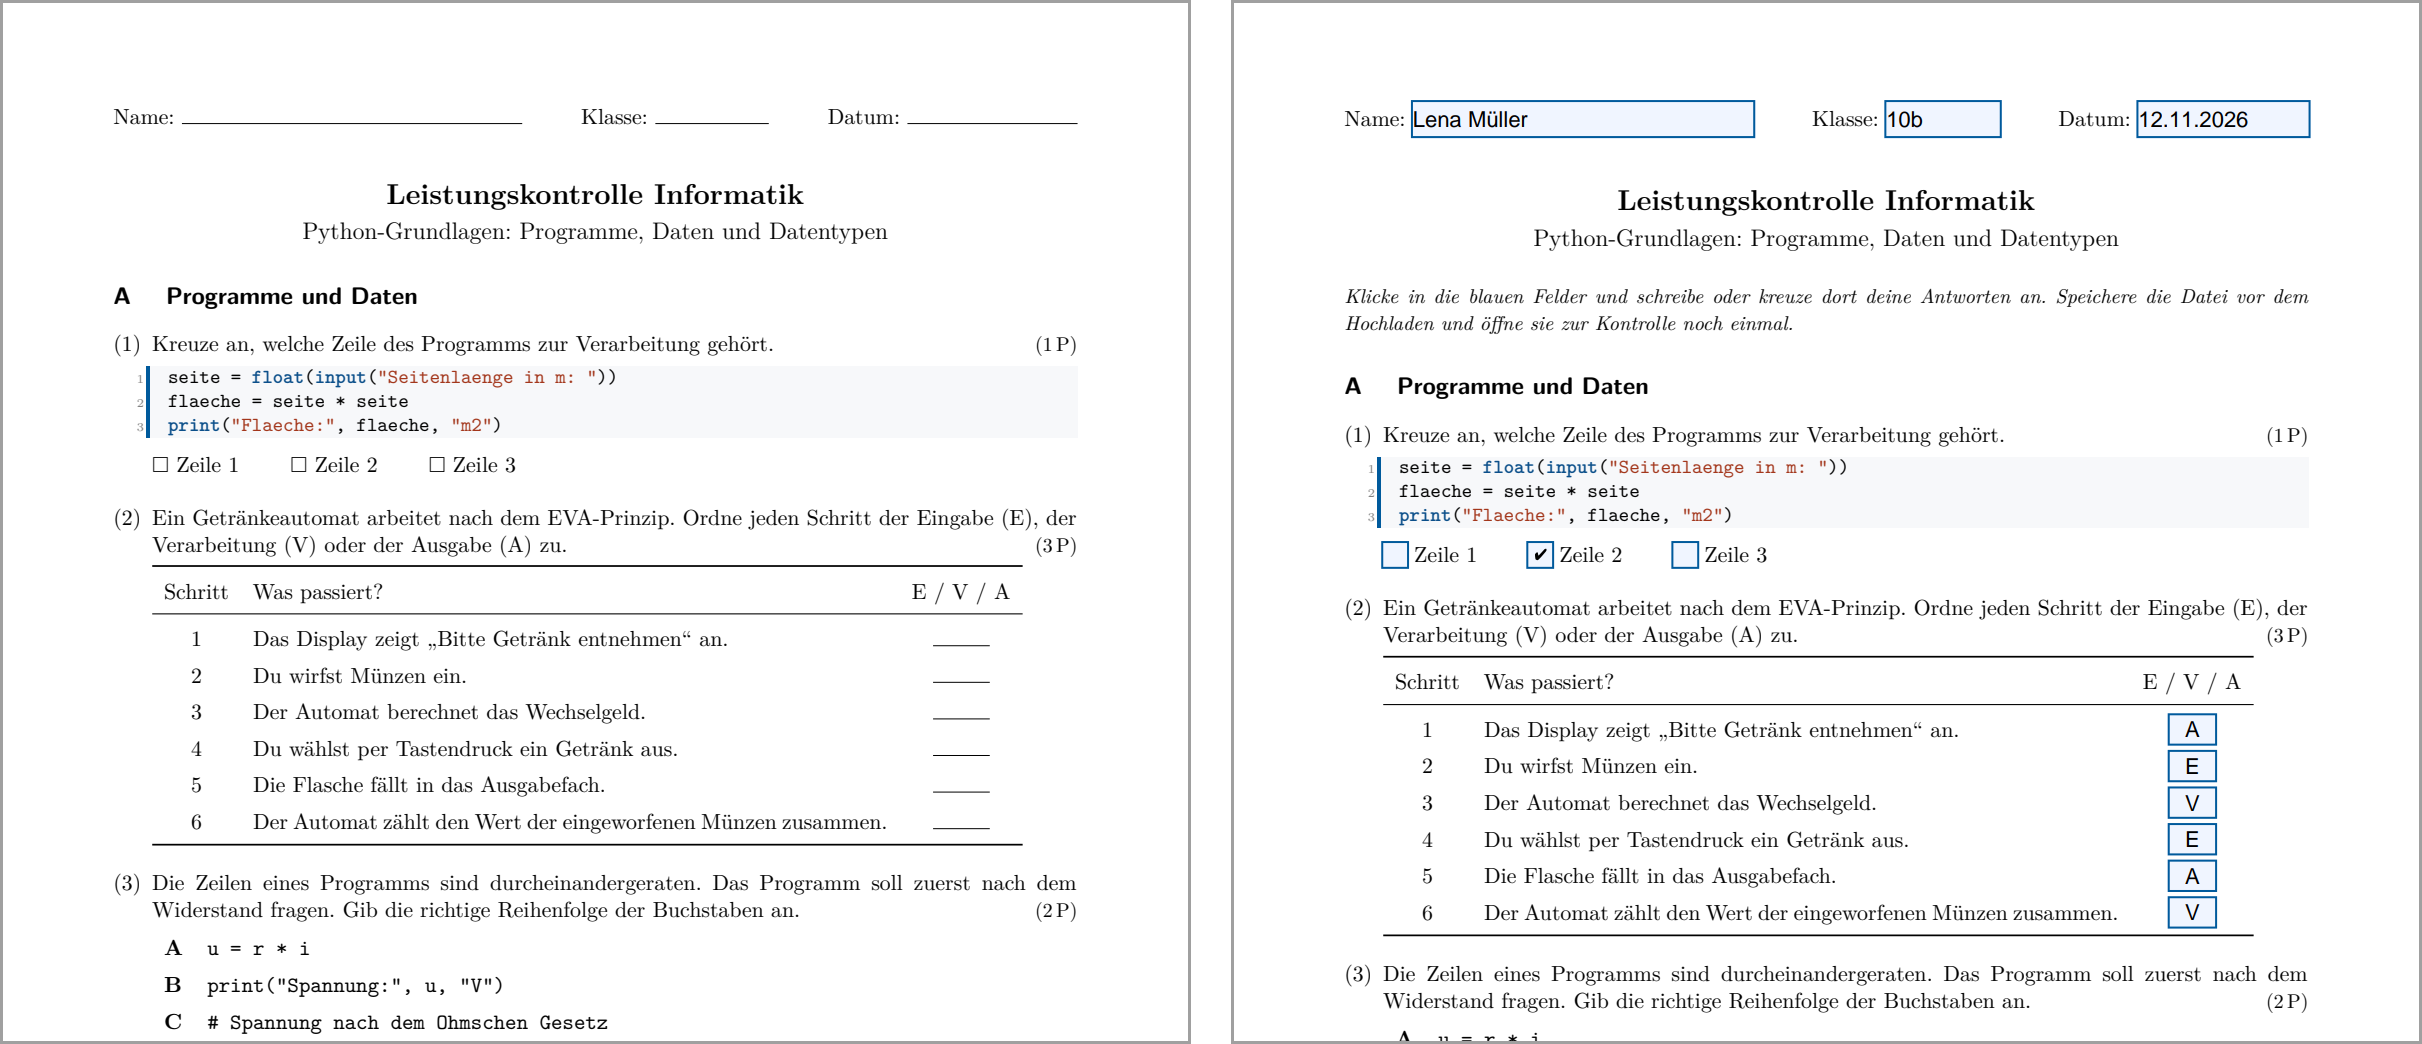
\includegraphics[width=\linewidth]{lk_vorher_nachher.png}\\[0.2cm]
	\small Links die Papierfassung, rechts die digitale Fassung, ausgefüllt
	und gespeichert in Chrome.
\end{center}

%%%%  UNTERKAPITEL 5.1  %%%%
\subsection{Der Umbau in fünf Schritten}

\begin{enumerate}[(1)]
	\item \textbf{Lösungsteil herausnehmen.} Er kommt in eine eigene Datei
	für die Lehrkraft. Alles, was im PDF steht, kann man auslesen, auch
	unsichtbar gemachten Text.
	\item \textbf{\texttt{Form} um den Inhalt legen} und
	\verb|\hypersetup{unicode=false}| ergänzen.
	\item \textbf{Ersetzen:} Kästchen durch \verb|\kreuz|, Schreiblücken durch
	\verb|\feld|, einzelne Buchstaben durch \verb|\zeichen|, Schreiblinien
	durch \verb|\antwort|.
	\item \textbf{Kopf:} Name, Klasse und Datum als Felder in den Text setzen.
	Die Kopfzeilen-Befehle wie \verb|\lk{10b}{Thema}| setzen Name und Punkte
	nur als Text in die Kopfzeile, dort gibt es keine Felder.
	\item \textbf{Hinweis für die Schülerinnen und Schüler} unter den Titel
	schreiben, wie bearbeitet und abgegeben wird.
\end{enumerate}

%%%%  UNTERKAPITEL 5.2  %%%%
\subsection{Kopf und Hinweis}

\begin{lstlisting}[style=latex]
Name: \feld[5.5cm]{name} \hfill Klasse: \feld[1.8cm]{klasse}
\hfill Datum: \feld[2.6cm]{datum}

{\small\itshape Klicke in die blauen Felder und schreibe oder kreuze dort
deine Antworten an. Speichere die Datei vor dem Hochladen und öffne sie zur
Kontrolle noch einmal.}
\end{lstlisting}

\begin{ausgabe}
Name: \feld[5.5cm]{name} \hfill Klasse: \feld[1.8cm]{klasse}
\hfill Datum: \feld[2.6cm]{datum}

{\small\itshape Klicke in die blauen Felder und schreibe oder kreuze dort
deine Antworten an. Speichere die Datei vor dem Hochladen und öffne sie zur
Kontrolle noch einmal.}
\end{ausgabe}


%%%%  UNTERKAPITEL 5.3  %%%%
\subsection{Eine Aufgabe vorher und nachher}

Auf Papier stand in der Aufgabe zu den Datentypen in jeder Zelle ein leeres
Kästchen \verb|\kasten| ($\square$). In der digitalen Fassung bekommt jedes
Kästchen einen eigenen Namen aus Aufgabe, Zeile und Spalte:

\begin{lstlisting}[style=latex]
\begin{tabular}{>{\ttfamily}l ccc}
  \toprule
  \textrm{Wert} & \texttt{int} & \texttt{float} & \texttt{str} \\
  \midrule
  15 & \kreuz{a7-1-int} & \kreuz{a7-1-float} & \kreuz{a7-1-str} \\
  1.72 & \kreuz{a7-2-int} & \kreuz{a7-2-float} & \kreuz{a7-2-str} \\
  "04109" & \kreuz{a7-3-int} & \kreuz{a7-3-float} & \kreuz{a7-3-str} \\
  \bottomrule
\end{tabular}
\end{lstlisting}

\begin{ausgabe}
\begin{tabular}{>{\ttfamily}l ccc}
  \toprule
  \textrm{Wert} & \texttt{int} & \texttt{float} & \texttt{str} \\
  \midrule
  15 & \kreuz{a7-1-int} & \kreuz{a7-1-float} & \kreuz{a7-1-str} \\
  1.72 & \kreuz{a7-2-int} & \kreuz{a7-2-float} & \kreuz{a7-2-str} \\
  "04109" & \kreuz{a7-3-int} & \kreuz{a7-3-float} & \kreuz{a7-3-str} \\
  \bottomrule
\end{tabular}
\end{ausgabe}


Eine Aufgabe mit Schreiblinien wird zu einem Antwortfeld:

\begin{lstlisting}[style=latex]
\begin{enumerate}[(1)]
  \setcounter{enumi}{4}
  \item Nenne vier Regeln, die du beim Festlegen eines Variablennamens in
  Python beachten musst. \hfill (4\,P)
  \antwort{a5}
\end{enumerate}
\end{lstlisting}

\begin{ausgabe}
\begin{enumerate}[(1)]
  \setcounter{enumi}{4}
  \item Nenne vier Regeln, die du beim Festlegen eines Variablennamens in
  Python beachten musst. \hfill (4\,P)
  \antwort{a5}
\end{enumerate}
\end{ausgabe}


Dieser Handreichung liegen bei:

\begin{itemize}
	\item \texttt{LK\_Python\_Grundlagen\_digital.tex}: die vollständige Leistungskontrolle,
	\item \texttt{vorlage\_lk\_digital.tex}: eine kurze Vorlage zum Weiterbauen.
\end{itemize}



%%%%  KAPITEL 6  %%%%
\section{Austeilen, bearbeiten, einsammeln}

%%%%  UNTERKAPITEL 6.1  %%%%
\subsection{Der Ablauf}

\begin{enumerate}[(1)]
	\item \textbf{Austeilen:} Die PDF-Datei (ohne Lösungen) über die
	Lernplattform bereitstellen, zum Beispiel als Datei in einer LernSax-Aufgabe.
	\item \textbf{Bearbeiten:} Die Schülerinnen und Schüler laden die Datei
	herunter, öffnen sie in einem Programm, das Formulare kann (siehe 6.2),
	und füllen die Felder aus.
	\item \textbf{Speichern und prüfen:} Die Datei speichern, schließen und
	noch einmal öffnen. Stehen die Antworten noch darin, hat das Speichern
	geklappt. Dieser Schritt ist der wichtigste, er kostet eine Minute und
	verhindert leere Abgaben.
	\item \textbf{Abgeben:} Die Datei mit dem eigenen Namen im Dateinamen
	hochladen, zum Beispiel \texttt{LK\_Mueller\_Lena.pdf}.
	\item \textbf{Bewerten:} Die Lehrkraft lädt die Abgaben herunter und
	korrigiert jede einzeln, zum Beispiel mit der Kommentar- oder Stiftfunktion
	des PDF-Programms, und gibt die korrigierte Datei zurück.
\end{enumerate}

Für eine Leistungskontrolle gelten dieselben Regeln wie auf Papier:
Bearbeitung im Raum, unter Aufsicht, in der festgelegten Zeit. Ob in dieser
Zeit andere Programme oder das Internet offen sind, lässt sich am Gerät nicht
erkennen. Das muss die Aufsicht regeln.

%%%%  UNTERKAPITEL 6.2  %%%%
\subsection{Welche Programme Formulare können}

Die Felder sind gewöhnliche PDF-Formularfelder ohne JavaScript. Getestet
wurde für diese Handreichung Folgendes:

\renewcommand{\arraystretch}{1.3}
\begin{tabular}{p{4.6cm} p{11cm}}
	\toprule
	\textbf{Programm} & \textbf{Ergebnis im Test} \\
	\midrule
	Chrome und Edge (PDFium) & Eintippen, Ankreuzen, Optionsfelder und
	Auswahllisten funktionieren, Umlaute und \texttt{ß} werden gespeichert und
	richtig wieder angezeigt. Getestet durch eine Simulation, die klickt und
	tippt wie ein Mensch. \\
	Poppler (z.\,B. Okular, Evince) & Text wird richtig angezeigt, ein Häkchen
	erscheint dort nur als schmaler Strich. \\
	\bottomrule
\end{tabular}

Adobe Acrobat Reader ist das Programm, für das PDF-Formulare ursprünglich
gemacht sind. Apple Vorschau, die Dateien-App auf dem iPad und
Notiz-Apps wie GoodNotes können ebenfalls Formularfelder ausfüllen, wurden für
diese Handreichung aber nicht getestet. Deshalb lohnt sich vor dem ersten
Einsatz eine \textbf{Probeabgabe}: In der Stunde davor ein kleines Formular
mit einem Feld jeder Art ausfüllen, speichern und hochladen lassen. Dann
weiß man, was auf den Geräten der Klasse funktioniert.



%%%%  KAPITEL 7  %%%%
\section{Antworten einsammeln mit Python (optional)}

Wer nicht jede Datei einzeln öffnen möchte, kann die Antworten aller Abgaben
in eine Tabelle holen. Das Skript \texttt{antworten\_einsammeln.py} liest alle
PDF-Dateien eines Ordners und schreibt eine CSV-Datei, die sich in Excel,
Numbers oder LibreOffice öffnen lässt: eine Zeile pro Abgabe, eine Spalte pro
Feld. Angekreuzte Kästchen erscheinen als \texttt{x}.

\begin{lstlisting}[style=latex, language=bash]
pip install pypdf
python3 antworten_einsammeln.py Abgaben_10b/
python3 antworten_einsammeln.py Abgaben_10b/ --aufgaben
\end{lstlisting}

Mit \texttt{--aufgaben} entsteht zusätzlich eine Textdatei, in der alle
Antworten zu einer Aufgabe untereinanderstehen. So lässt sich Aufgabe für
Aufgabe korrigieren, was den Maßstab über die ganze Klasse gleich hält. Ein
Ausschnitt mit zwei Testabgaben:

\begin{lstlisting}[style=latex, language={}]
===== a8-c =====
LK_Lena_Mueller.pdf:
    2.5
LK_Tom_Schulze.pdf:
    2,5
\end{lstlisting}

Bewertet wird weiterhin von der Lehrkraft. Das Skript sortiert nur.



%%%%  KAPITEL 8  %%%%
\section{Tipps und Stolpersteine}

Alles in diesem Kapitel wurde ausprobiert.

\begin{itemize}
	\item \textbf{Felder in Tabellen werden zu hoch.} Ein nacktes
	\verb|\TextField| oder \verb|\CheckBox| übernimmt die Höhe der
	Tabellenzeile. Lösung: das Feld in \verb|\raisebox| oder \verb|\hbox|
	packen, wie es die Kurzbefehle tun.
	\item \textbf{Optionsfelder funktionieren nicht.} Fehlt in der Präambel
	die Zeile\newline \verb|\hypersetup{unicode=false}|, erzeugt \texttt{hyperref} 7.01h
	Werte wie \verb|\376\377\000z\0001| statt \texttt{z1}. Chrome speichert die
	Auswahl dann zwar, aber genau als diesen Zeichensalat, und beim Einsammeln
	(Kapitel 7) lässt sich nicht mehr ablesen, welche Option gewählt wurde.
	\item \textbf{Unterstriche verschwinden aus Feldnamen.} Bindestriche
	verwenden.
	\item \textbf{\texttt{\textbackslash Reset} leert alle Felder}, nicht nur
	die in der Nähe des Knopfes, auch über mehrere \texttt{Form}-Umgebungen
	hinweg. In einer Leistungskontrolle hat so ein Knopf nichts verloren.
	\item \textbf{Lösungen nie ins Schülerdokument}, auch nicht weiß auf weiß
	oder auf einer ausgeblendeten Ebene. Text in einem PDF lässt sich immer
	herauskopieren.
	\item \textbf{Mehrere \texttt{Form}-Umgebungen} in einem Dokument sind
	möglich, eine einzige um den ganzen Inhalt ist aber übersichtlicher.
	\item \textbf{Platz einplanen:} Was über ein mehrzeiliges Feld hinausgeht,
	ist am Bildschirm über Scrollen erreichbar, auf dem Ausdruck aber
	abgeschnitten.
\end{itemize}



%%%%  KAPITEL 9  %%%%
\section{Befehlsreferenz}

%%%%  UNTERKAPITEL 9.1  %%%%
\subsection{Kurzbefehle aus der newcommands.tex}

\renewcommand{\arraystretch}{1.3}
\begin{tabular}{p{5.6cm} p{10cm}}
	\toprule
	\textbf{Befehl} & \textbf{Wirkung} \\
	\midrule
	\verb|\feld[B]{Name}| & einzeiliges Textfeld auf der Grundlinie, Breite B (Standard 2,4\,cm) \\
	\verb|\zeichen{Name}| & Feld für genau ein Zeichen, zentriert, 0,8\,cm breit \\
	\verb|\kreuz{Name}| & Ankreuzkästchen, 0,42\,cm \\
	\verb|\antwort[H]{Name}| & mehrzeiliges Feld über die ganze Breite, Höhe H (Standard 3,2\,cm) \\
	\bottomrule
\end{tabular}

%%%%  UNTERKAPITEL 9.2  %%%%
\subsection{Befehle und Optionen von hyperref}

\begin{tabular}{p{5.6cm} p{10cm}}
	\toprule
	\textbf{Befehl / Option} & \textbf{Wirkung} \\
	\midrule
	\verb|\begin{Form}| & Umgebung, in der alle Felder stehen \\
	\verb|\TextField[...]{Text}| & Textfeld, \texttt{Text} wird als Beschriftung davorgesetzt \\
	\verb|\CheckBox[...]{Text}| & Ankreuzkästchen \\
	\verb|\ChoiceMenu[radio,...]|\newline\verb|  {}{a=1,b=2}| & Optionsfelder, \texttt{Beschriftung=Wert} \\
	\verb|\ChoiceMenu[combo,|\newline\verb|  popdown,...]{}{E,V,A}| & Auswahlliste \\
	\verb|\Reset{Text}| & Knopf, der alle Felder leert \\
	\midrule
	\texttt{name=} & Feldname, im Dokument eindeutig, ohne Unterstrich \\
	\texttt{width=}, \texttt{height=} & Breite und Höhe \\
	\texttt{charsize=} & Schriftgröße der Eingabe, z.\,B. \texttt{11pt} \\
	\texttt{value=} & vorgetragener Text \\
	\texttt{default=} & Startwert, bei \texttt{radio} leer lassen: \texttt{default=} \\
	\texttt{multiline=true} & mehrzeiliges Textfeld \\
	\texttt{maxlen=} & höchstens so viele Zeichen \\
	\texttt{align=} & 0 links, 1 zentriert, 2 rechts \\
	\texttt{bordercolor=}, \texttt{backgroundcolor=} & Rand- und Hintergrundfarbe als \texttt{\{r g b\}}, Werte 0 bis 1 \\
	\texttt{print} & Feld wird mitgedruckt \\
	\bottomrule
\end{tabular}

Die vollständige Liste steht in der Dokumentation von \texttt{hyperref}
(\texttt{texdoc hyperref}, Abschnitt \enquote{Forms}).



%%%%  KAPITEL 10  %%%%
\section{Zusammenfassung}

\begin{itemize}
	\item Formularfelder erzeugt \texttt{hyperref}, alle Felder stehen in
	\verb|\begin{Form} ... \end{Form}|, dazu \verb|\hypersetup{unicode=false}|.
	\item Für Arbeitsblätter und Leistungskontrollen reichen vier
	Kurzbefehle:\newline \verb|\feld|, \verb|\zeichen|, \verb|\kreuz| und
	\verb|\antwort|.
	\item Jedes Feld braucht einen eindeutigen Namen ohne Unterstrich, am
	besten nach Aufgabennummer.
	\item Eine Papierfassung wird digital, indem man Kästchen, Lücken und
	Linien durch Felder ersetzt und die Lösungen herausnimmt.
	\item Vor dem ersten Einsatz eine Probeabgabe auf den Geräten der Klasse
	machen.
\end{itemize}

Für den Unterricht heißt das: Dieselbe Datei, aus der die Papierfassung
entsteht, liefert mit wenigen Änderungen eine digitale Fassung. Die
Schülerinnen und Schüler brauchen nur ein PDF-Programm, die Lehrkraft
korrigiert so individuell wie auf Papier und hat die Abgaben trotzdem
geordnet auf der Lernplattform.

\end{Form}
\end{document}
